\documentclass[dvipsnames]{beamer}
\beamertemplatenavigationsymbolsempty
\usetheme{Boadilla}
\usefonttheme[onlymath]{serif}

\usepackage{amsmath}
\usepackage{bm}
\usepackage{bbm}
\usepackage{mathrsfs}
\usepackage{mathtools}
\usepackage[cal=boondoxo]{mathalpha}

% Change horizontal spacing
\setlength{\tabcolsep}{3pt}

\usepackage[none]{hyphenat} % no hyphenation

\usepackage{array}

\usepackage{cancel}

\usepackage[style=authoryear,maxcitenames=2,backend=biber,citetracker=true]{biblatex}
\addbibresource{references.bib}

\usepackage{verbatim}

\newcommand{\credit}[2]{\par\hfill \footnotesize #1 credit:~\itshape\citeauthor{#2} (\citeyear{#2})}
\renewcommand{\cite}[1]{(\citeauthor{#1}, \citeyear{#1})}
\newcommand{\matr}[1]{#1}

\newcommand{\red}[1]{{\color{red} #1}}

\title[XAI with Shapley Value]
{Explainable Machine Learning\\with Shapley Value}
%\subtitle{}
\author{Gianmarco Midena}
\institute{Aalto University}
\date{12 March 2024}

\begin{document}
\begin{frame}
\titlepage
\end{frame}

%\begin{frame}{Outline}
%\tableofcontents
%\end{frame}

\begin{frame}{Introduction}
	\begin{itemize}
		\item How each feature affects the prediction of a data point.
	\end{itemize}
\end{frame}

\begin{frame}{Example - Probability of Cervical Cancer for a Woman}
	\begin{center}
		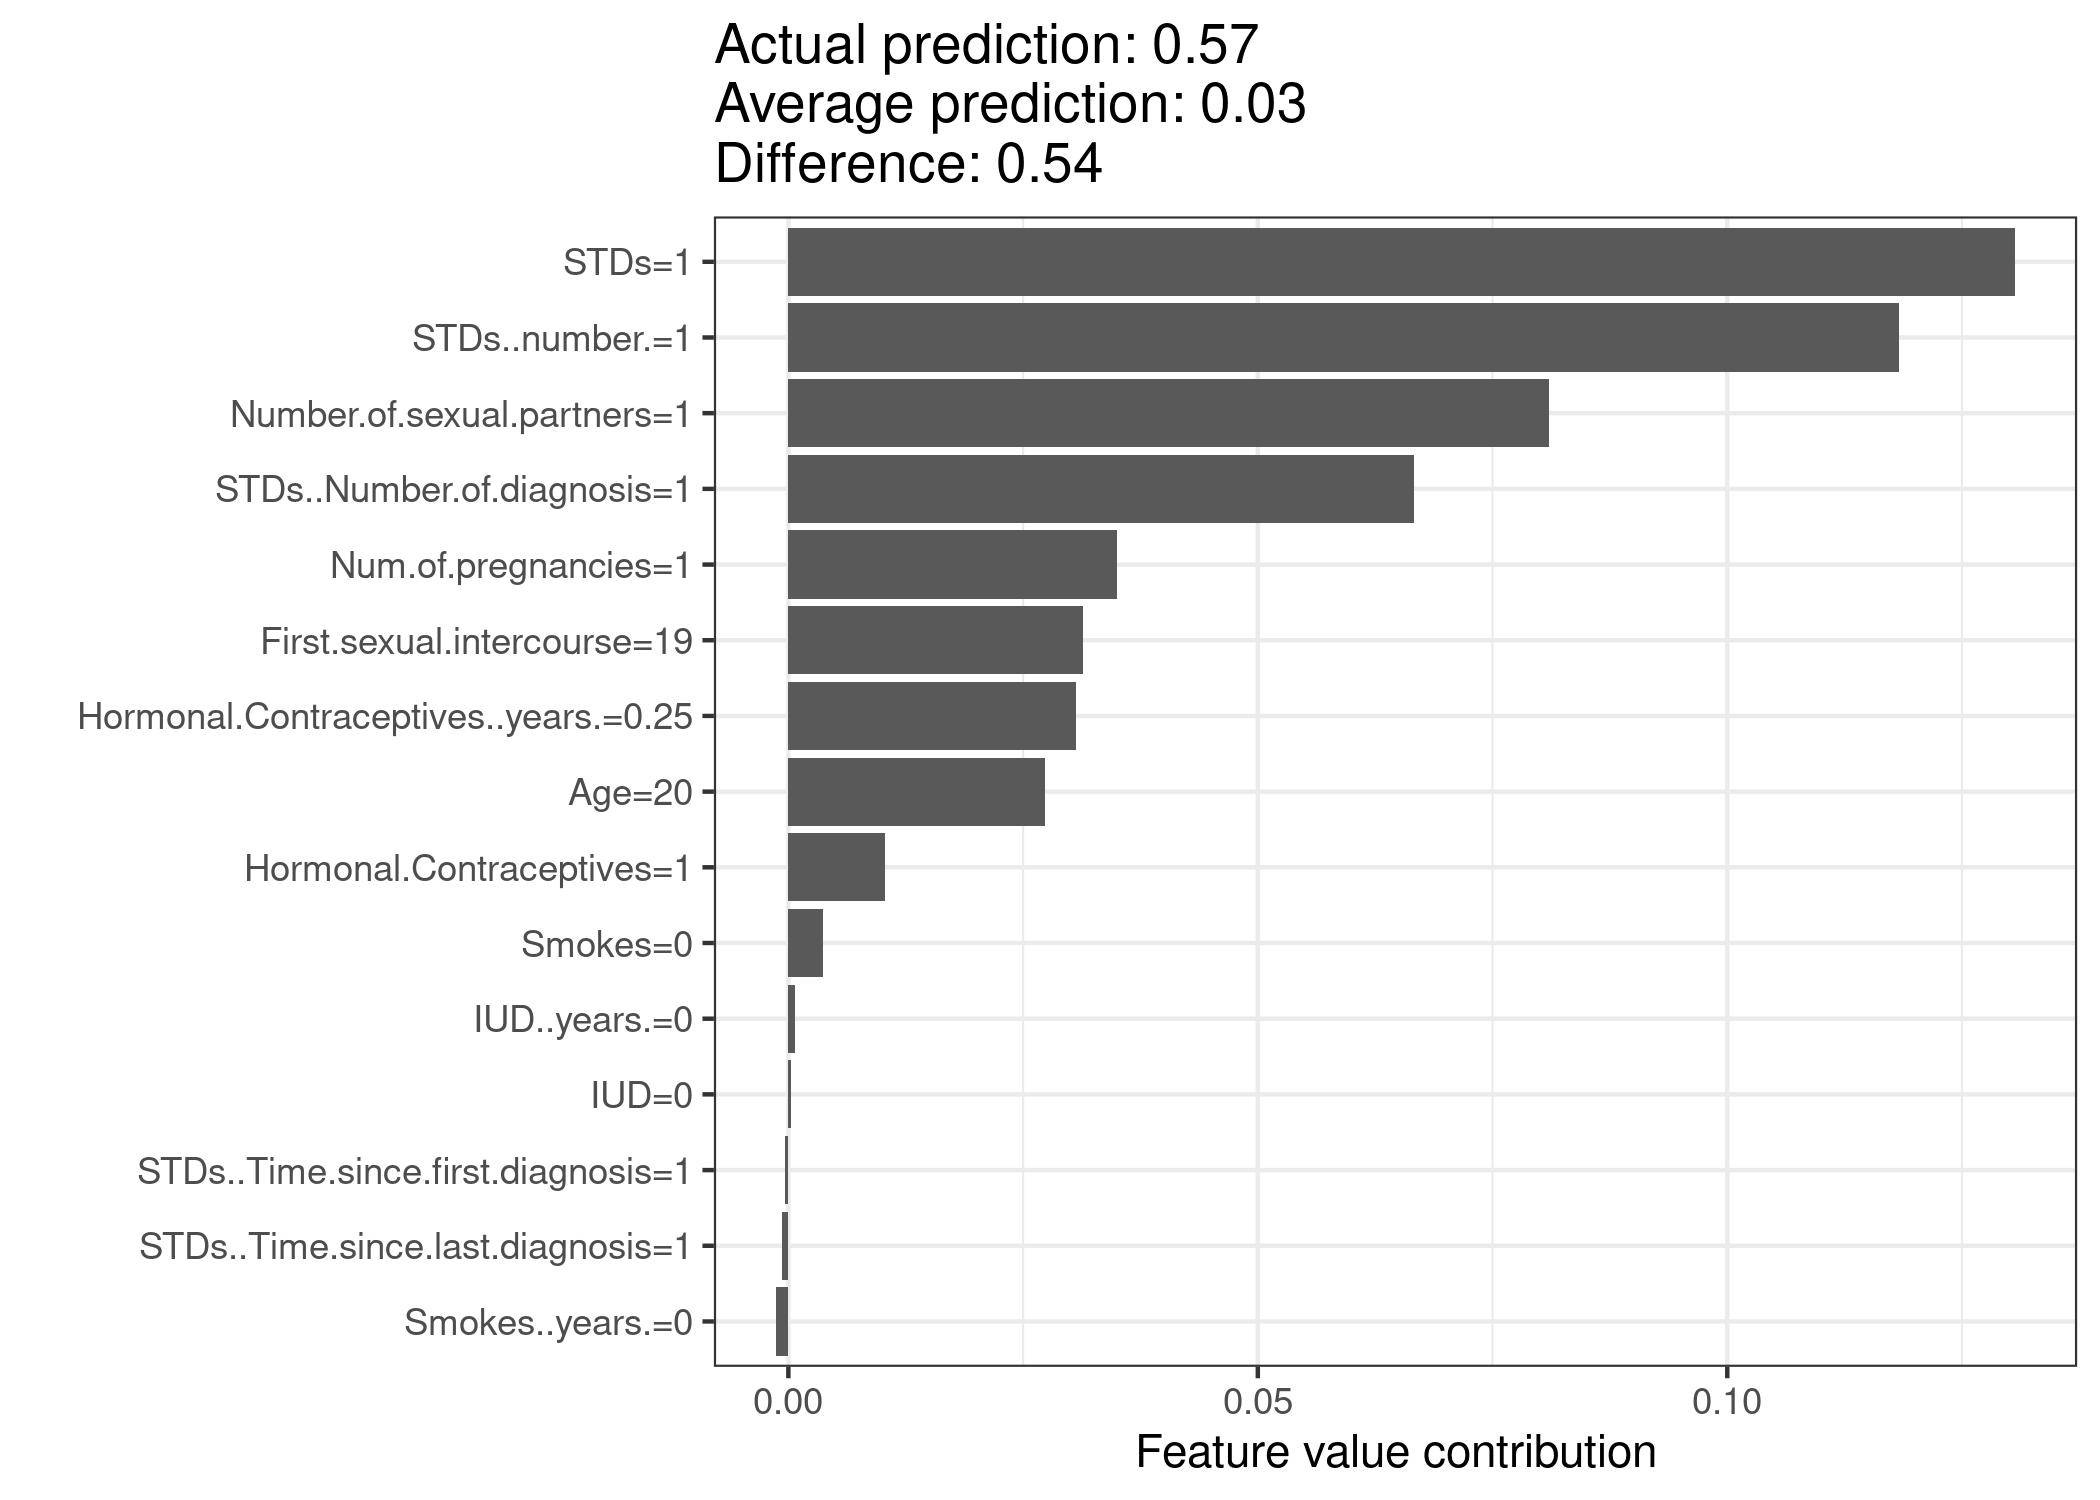
\includegraphics[scale=0.6]{images/shapley-cervical-plot-1.jpeg}
	\end{center}
\credit{Image}{molnar2020interpretable}
\end{frame}

\begin{frame}{Risk Factors for Cervical Cancer\footnotemark}
\begin{itemize}
	\item Has patient ever had a sexually transmitted disease (STD) [binary]
	\item Number of sexual partners
	\item Number of STD diagnoses
	\item Number of pregnancies
	\item First sexual intercourse (age in years)
	\item Hormonal contraceptives (in years)
	\item Age in years
	\item Hormonal contraceptives [binary]
	\item Smokes (binary)
	\item Number of years with an intrauterine device (IUD)
	\item Intrauterine device (IUD) [binary]
	\item Time since first STD diagnosis
	\item Time since last STD diagnosis
	\item Smokes (in years)
\end{itemize}
\footnotetext[1]{\citeauthor{risk_factors_dataset} (\citeyear{risk_factors_dataset})}
\end{frame}

\begin{frame}{Example - Number of Rented Bikes for a Day}
	\begin{center}
		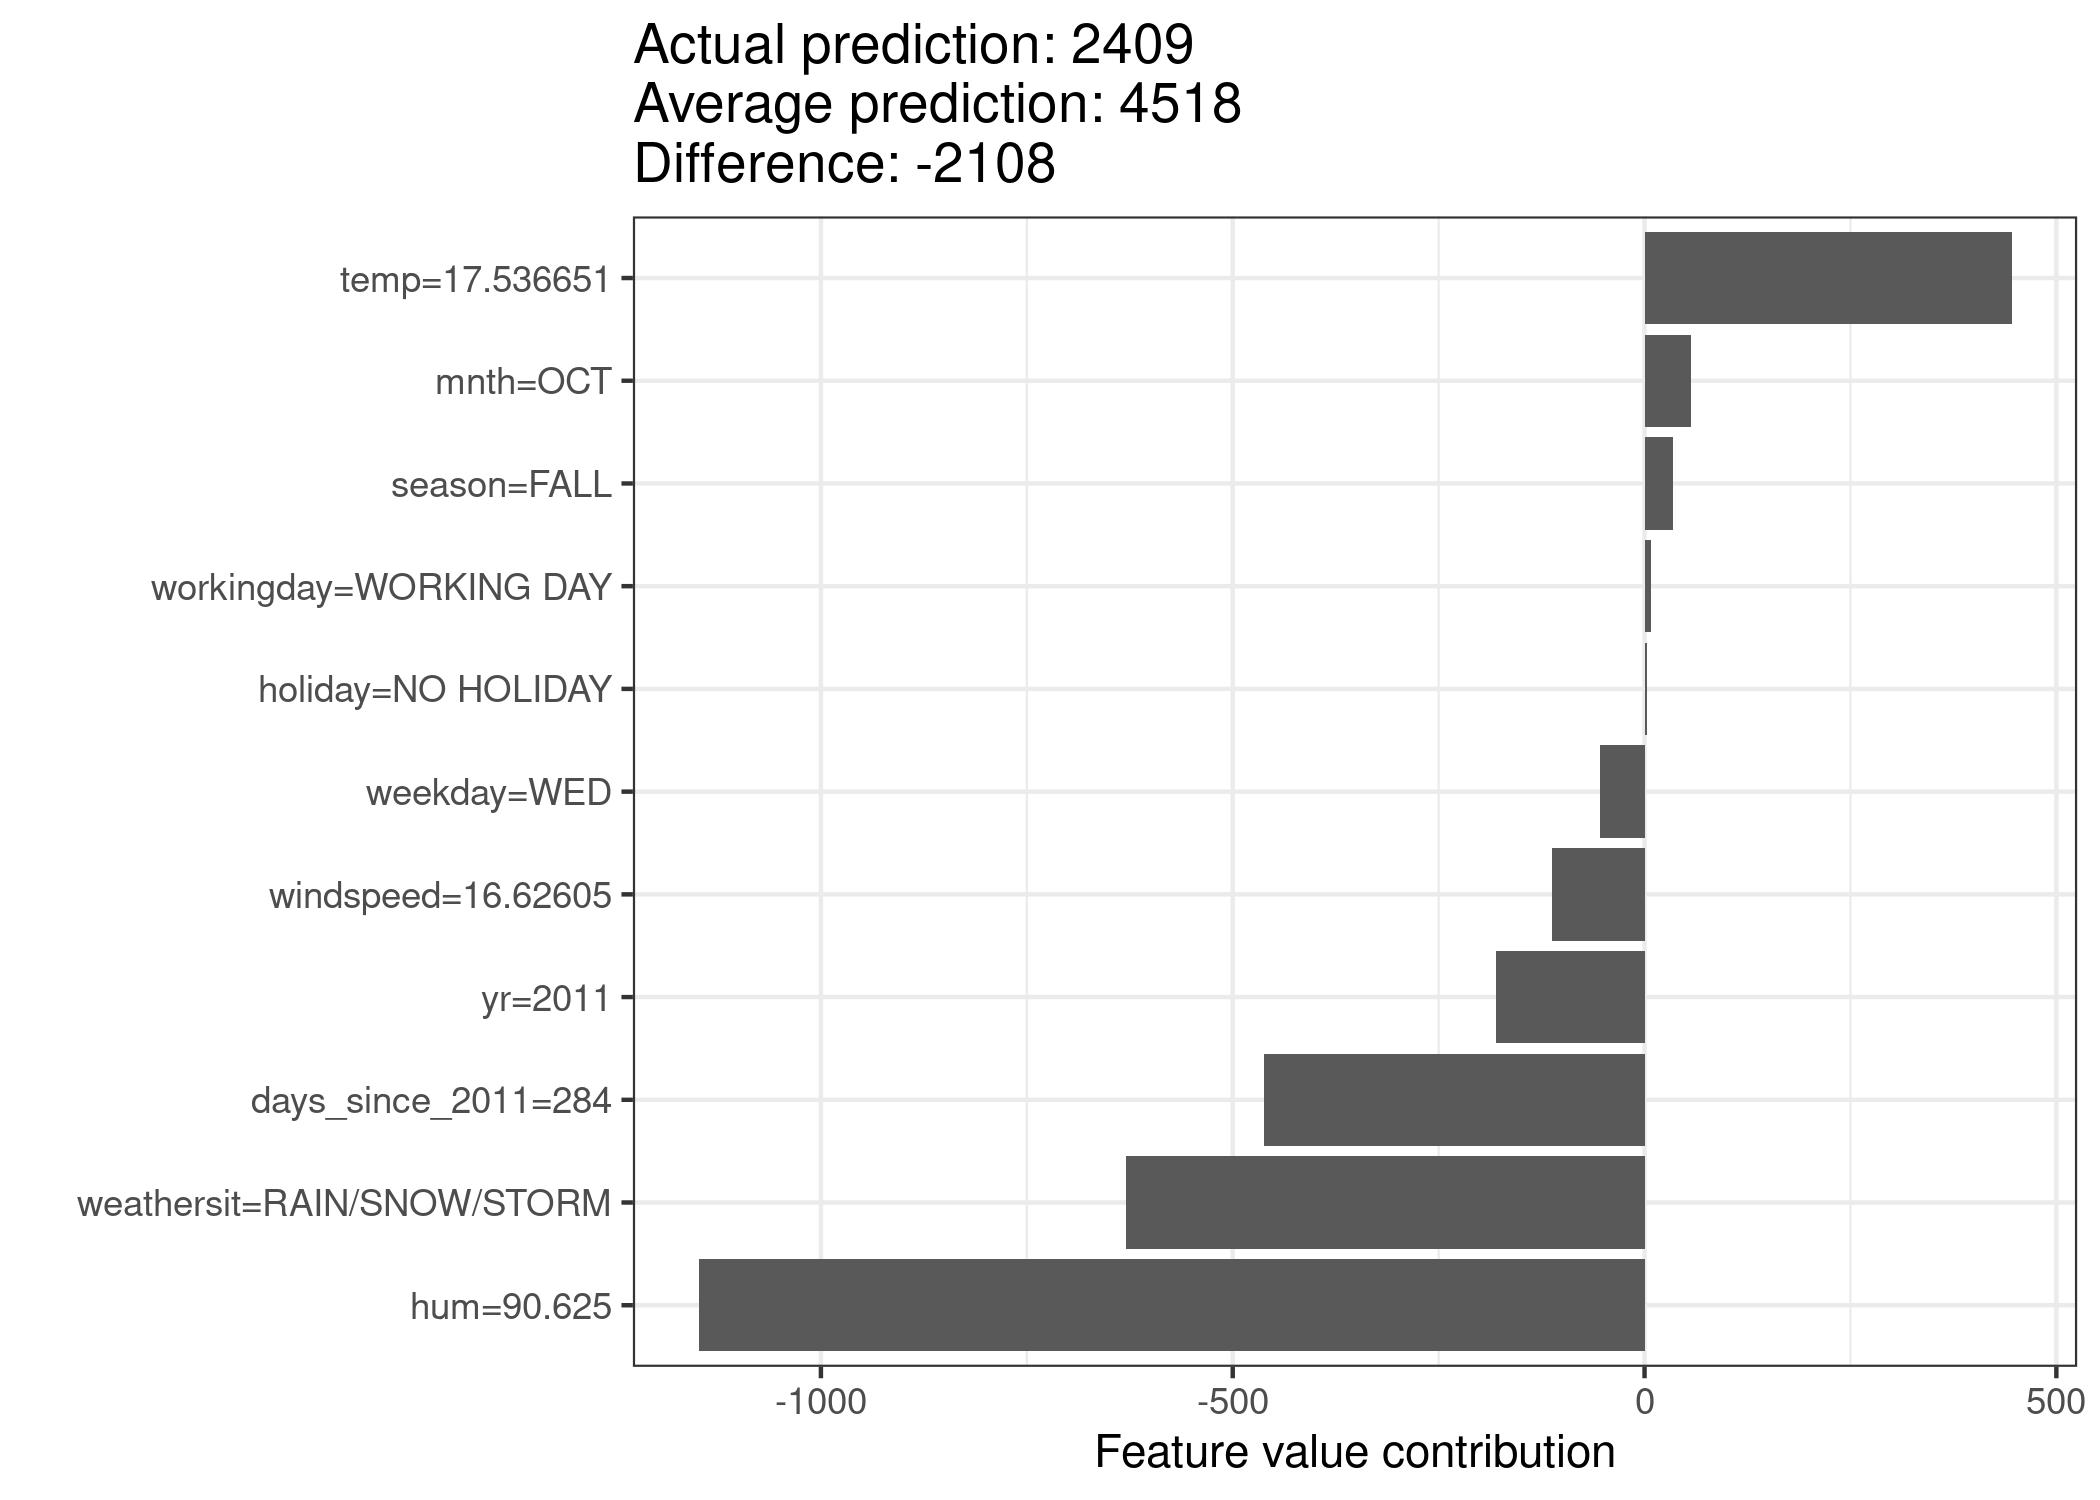
\includegraphics[scale=0.6]{images/shapley-bike-plot-1.jpeg}
	\end{center}
	\credit{Image}{molnar2020interpretable}
\end{frame}

\begin{frame}{Bike Rental Features\footnotemark}
	\begin{itemize}
		\item Temperature in degrees Celsius
		\item Season: spring, summer, fall or winter
		\item Working day or weekend
		\item Holiday or not
		\item Wind speed in km per hour
		\item Year: 2011 or 2012
		\item Nr. days since 01.01.2011 (the first day in the dataset).
		\item Weather situation:
		\begin{enumerate}[a]
			\item clear, few clouds, partly cloudy, cloudy
			\item mist + clouds, mist + broken clouds, mist + few clouds, mist
			\item light snow, light rain + thunderstorm + scattered clouds, light rain + scattered clouds
			\item heavy rain + ice pallets + thunderstorm + mist, snow + mist
		\end{enumerate}
		\item Relative humidity percentage
	\end{itemize}
	\footnotetext[2]{\citeauthor{bike_sharing_dataset} (\citeyear{bike_sharing_dataset})}
\end{frame}

\begin{frame}{Linear Model}
	\begin{itemize}
		\item prediction
		\begin{equation}
			\hat{f}(\bm{x})=w_0+w_1 x_{1} + \dots + w_p x_ p
		\end{equation}
		\begin{itemize}
			\item $\bm{x}$: data instance
			\item $x_j$: value of feature $j$
			\item $w_j$: weight corresponding to feature $j$
			\item $p$: nr. features
		\end{itemize}
		\item easy to calculate \emph{individual effects}
	\end{itemize}
\end{frame}
\begin{frame}{Linear Model - Feature Contribution}
	\begin{itemize}
		\item $j$-th feature contribution $\phi_j$
		\begin{align}
			\begin{split}
				\phi_j(\hat{f})
				&=w_{j}x_j-E(w_{j}X_{j})\\
				&=w_{j}x_j-w_{j}E(X_{j})
			\end{split}
		\end{align}
		\begin{itemize}
			\item $j$-th feature effect minus average $j$-th feature effect
			\item $E(w_{j}X_{j})$: mean effect estimate for feature $j$
		\end{itemize}
	\end{itemize}
\end{frame}
\begin{frame}{Linear Model - Total Feature Contribution}
	\begin{align}
		\begin{split}
			\sum_{j=1}^{p}\phi_j(\hat{f}) =&\sum_{j=1}^p(w_{j}x_j-E(w_{j}X_{j}))\\
			=&(w_0+\sum_{j=1}^pw_{j}x_j)-(w_0+\sum_{j=1}^{p}E(w_{j}X_{j}))\\
			=&\hat{f}(\bm{x})-E(\hat{f}(X))
		\end{split}
	\end{align}
	\begin{itemize}
		\item predicted value minus average predicted value
		\item $E(w_{j}X_{j})$: mean effect estimate for feature $j$
		\item $\phi_j$: $j$-th feature contribution
		\item $\bm{x}$: data instance
		\item $x_j$: value of feature $j$
		\item $w_j$: weight corresponding to feature $j$
		\item $p$: nr. features
	\end{itemize}
\end{frame}

\begin{frame}{Feature Contribution in General}
	\begin{itemize}
		\item \emph{Can we do the same for any type of model?}
		\\It would be great to have this as a model-agnostic tool.
		\item \red{Since we usually do not have similar weights in other model types, we need a different solution.}
		\item possible solution: \underline{Shapley value}
		\begin{itemize}
			\item field: Cooperative Game Theory
		\end{itemize}
	\end{itemize}
\end{frame}

\begin{frame}{Shapley Values - Feature Contribution}
\begin{equation}
	\phi_j(val_{\bm{x}})=\sum_{S\subseteq\{1,\ldots,p\} \backslash \{j\}}\frac{|S|!\left(p-|S|-1\right)!}{p!}\left(val_{\bm{x}}\left(S\cup\{j\}\right)-val_{\bm{x}}(S)\right)
\end{equation}
\begin{itemize}
	\item Contribution of $j$-th feature value to the prediction (\emph{payout})
	\item Normalized: weighted and summed over all possible feature combinations
	\item $j$-th feature value
	\item $val_{\bm{x}}(S)$: value of players in $S$ %\red{to explain $\bm{x}$}
	\item $S$: a subset of features used in the model (\emph{coalition})
	\item $\bm{x}$: vector of feature values of an instance to be explained
	\item $p$: nr. features
\end{itemize}
\end{frame}

\begin{frame}{Shapley Value - The Value Function}
\begin{equation}
	val_{x}(S)=\int\hat{f}(x_{1},\ldots,x_{p})d\mathbb{P}_{x\notin{}S}-E_X(\hat{f}(X))
\end{equation}
\begin{itemize}
	\item Payout function for coalitions of players (feature values)
	\item Predicts feature values in $S$
	\item Marginalizes over features that are not in $S$
	\item Multiple integrations for each feature that is not in $S$
\end{itemize}
\end{frame}

\begin{frame}{Shapley Value - The Value Function - Example}
\begin{equation}
val_{x}(\{1,3\})=\int_{\mathbb{R}}\int_{\mathbb{R}}\hat{f}(x_{1},X_{2},x_{3},X_{4})d\mathbb{P}_{X_2X_4}-E_X(\hat{f}(X))
\end{equation}
\begin{itemize}
	\item $S = \{1,3\}$: features in coalition
	\item $p = 4$: tot. model features
\end{itemize}
\end{frame}

\begin{frame}{Shapley Value - Properties}
	\begin{enumerate}
		\item Dummy
		\item Efficiency
		\item Symmetry
		\item Additivity
	\end{enumerate}
	\begin{itemize}
		\item Axioms
		\item Fair Payout
	\end{itemize}
\end{frame}
\begin{frame}{Shapley Value - Dummy}
	If
	\begin{equation}
		val_{\bm{x}}(S\cup\{j\})=val(S)
	\end{equation}
	for all
	\begin{equation*}
		S\subseteq\{1,\ldots,p\}
	\end{equation*}
	then
	\begin{equation*}
		\phi_j=0
	\end{equation*}
	\begin{itemize}
		\item A feature $j$ that does not change the predicted value - regardless of which coalition of feature values it is added to - should have a Shapley value of 0.
	\end{itemize}
\end{frame}
\begin{frame}{Shapley Value - Efficiency}
	\begin{equation}
		\sum\nolimits_{j=1}^p\phi_j=\hat{f}(\bm{x})-E_X(\hat{f}(X))
	\end{equation}
	\begin{itemize}
		\item Feature contributions must \emph{sum} up to prediction for $\bm{x}$ \emph{minus} average prediction
	\end{itemize}
\end{frame}
\begin{frame}{Shapley Value - Symmetry}
	If
	\begin{equation}
		val_{\bm{x}}(S \cup \{j\})=val(S\cup\{k\})
	\end{equation}
	for all
	\begin{equation*}
		S\subseteq\{1,\ldots, p\} \backslash \{j,k\}
	\end{equation*}
	then
	\begin{equation*}
		\phi_j=\phi_k
	\end{equation*}
	\begin{itemize}
		\item The contribution of two feature values $j$ and $k$ should be the same, 
		\\if they contribute equally to all possible coalitions.
	\end{itemize}
\end{frame}
\begin{frame}{Shapley Value - Additivity}
	If
	\begin{equation}
		val_{\bm{x} + \bm{y}}(S)=val_{\bm{x}}(S) + val_{\bm{y}}(S)
	\end{equation}
	for all
	\begin{equation*}
		\bm{x}, \bm{y} \in \mathcal{X},\; S\subseteq\{1,\ldots, p\}
	\end{equation*}
	then
	\begin{equation*}
		\phi(\bm{x} + \bm{y})=\phi(\bm{x}) + \phi(\bm{y})
	\end{equation*}
	%\begin{equation}
	%	\phi_j+\phi_j^{+}
	%\end{equation}
	\begin{itemize}
		\item Combined payouts
		\item Example: Random forest = average of many decision trees
		\begin{itemize}
			\item Prediction = average prediction in decision trees
			\item Feature contribution = average feature contribution in decision trees
		\end{itemize}
	\end{itemize}
\end{frame}


\begin{frame}[fragile]{Some Implementations}
	\begin{itemize}
		\item \verb|fastshap| (R)~\cite{jethani2021fastshap}
		\item \verb|iml| (R)~\cite{molnar2018iml}
		\item \verb|breakDown| (R)~\cite{staniak2018explanations}
		\item \verb|Shapley.jl| (Julia)~\footnotemark
	\end{itemize}
	\footnotetext[4]{\href{https://gitlab.com/ExpandingMan/Shapley.jl}{https://gitlab.com/ExpandingMan/Shapley.jl}}
\end{frame}

\begin{frame}{Shapley Value in Short}
	\begin{itemize}
		\item Permutation-based
		\item Model-agnostic
		\item Solid theory
		\item Full-explanation
		\begin{itemize}
			\item All the features
			\item Non sparse (proper subset of features)
		\end{itemize}
		\item Model-free
		\item Data access or generation
		\item Building block in SHAP~\cite{lundberg2017unified}
	\end{itemize}
\end{frame}

\section{References}
\begin{frame}[allowframebreaks]
\frametitle{References}
\printbibliography
\end{frame}

\end{document}